\documentclass[11pt, spanish]{article}

\usepackage[spanish]{babel}
\selectlanguage{spanish}
\usepackage[utf8]{inputenc}
\usepackage{graphicx}
\usepackage[pdftex]{graphicx}
\usepackage{fancyhdr}
\usepackage{amsmath, amssymb}
\usepackage{enumerate}


\pagestyle{fancy}
\fancyhf{}
\rhead{201111578 \\ 201317343}
\lhead{Sebastián Valencia Calderón \\ Edgar Daniel Gómez}
\rfoot{\thepage}

\begin{document}
\section{Cálculo de probabilidades de eventos (Diagrama de Venn)}

Petrocol es una multinacional dedicada a la producción de petróleo que opera en Colombia. El plan estratégico de la compañia contempla la inversión en exploración y explotación de nuevos yacimientos. En este plan existen dos alternativas de inversión que son atractivas económicamente para la junta directiva. La primera alternativa (\textbf{Alternativa A}) consiste en explorar y explotar las reservas de petróleo ubicadas en aguas profundas del caribe colombiano. La segunda alternativa (\textbf{Alternativa B}) consiste en explorar y explotar las reservas petroleras distribuidas en los municipios de Arauca y Casanare. Petrocol reconoce que, por restricciones presupuestarias, no cuenta con los recursos operativos (maquinaria y equipo) suficientes para implementar las dos alternativas de manera simultánea. Esto implica que se debe elegir cuál de las dos alternativas se implementará primero. Adicionalmente, la junta directiva está considerando varias alternativas de financiación para respaldar el proyecto que se elija. Estas alternativas de financiación son:

\begin{itemize}
\item \textbf{Crédito Bancario}: obtener el 100\% de los recursos económicos que requiere la alternativa a través de un crédito.
\item \textbf{Exceso de Caja}: financiar la totalidad del proyecto de contado, a partir del exceso de caja que se obtuvo el año anterior.
\item \textbf{Emisión de Acciones}: realizar una emisión de acciones para recaudar el capital necesario de la alternativa.
\end{itemize}

Con el fin de analizar las dos alternativas de inversión, la junta directiva realizó una encuesta a 5000 accionistas de la compañía, seleccionados de manera aleatoria. La junta directiva espera que la encuesta les permita evaluar las preferencias de los accionistas en cuanto al proyecto que se debería realizar y al método de financiación que considerarían apropiado. Los resultados de la encuesta arrojaron la siguiente información:

\begin{itemize}
\item 2320 accionistas están de acuerdo con la inversión en la alternativa A.
\item 745 accionistas no están de acuerdo con el plan estratégico de la junta directiva.
\item 1690 accionistas están de acuerdo en invertir en la alternativa A y financiarla a partir de un crédito bancario. De esos 1690, hay 865 que también aceptarían utilizar el exceso de caja
como forma de financiación.
\item 185 accionistas están de acuerdo con invertir en la alternativa B y consideran que la opción 3 es el único método de financiación adecuado.
\item De los accionistas que apoyan la alternativa B y que consideran apropiado utilizar el exceso
de caja, hay 145 que también estarían dispuestos a aceptar una emisión de acciones, pero
que no aceptarían solicitar un crédito bancario.
\item 1285 accionistas están de acuerdo con invertir en la alternativa B y financiarla a partir de un
crédito bancario. De estos 1285, 610 también estarían de acuerdo con una emisión de acciones; y de los 610, son 200 los accionistas que también estarían de acuerdo con utilizar el exceso de caja.
\item De los 1285 accionistas que financiarían la alternativa B con un crédito bancario, hay 315 que estarían también de acuerdo con utilizar el exceso de caja pero no estarían de acuerdo con una emisión de acciones.
\item De los accionistas que apoyan la alternativa A, ninguno de ellos considera que una emisión de acciones es un método viable de financiación.

\end{itemize}

Con base en la información anterior, de respuesta a los siguientes literales:

\begin{enumerate}[(a)]

\item Con base en la información anterior, mencione los eventos que se presentan en la situación expuesta.\\

Los eventos presentados en la descripción del problema anterior, incluyen los eventos asociados al lugar de a inversión y los tipos de inversión. Es decir, los eventos probables de éste experimento es el producto cruz de las alternativas y los métodos de inversión ($CB$ representa crédito bancario, $EC$, emisión de caja y $EA$ emisión de acciones). Sin embago, es necesarios tener en cuneta que los accionistas que apoyan la alternativa A no desean financiar el proyecto através de emisión de caja:

$$\Omega = \left[A, B \right] \times \left[CB, EC, EA \right]$$
$$\Omega = \left\{ (A, CB), (A, EA), (B, CB), (B, EC), (B, EA)\right\}$$

\pagebreak

\item Realice un diagrama de Venn que indique la cantidad de accionistas que pertenecen a cada evento.\\

\begin{figure}[h]
\centering
	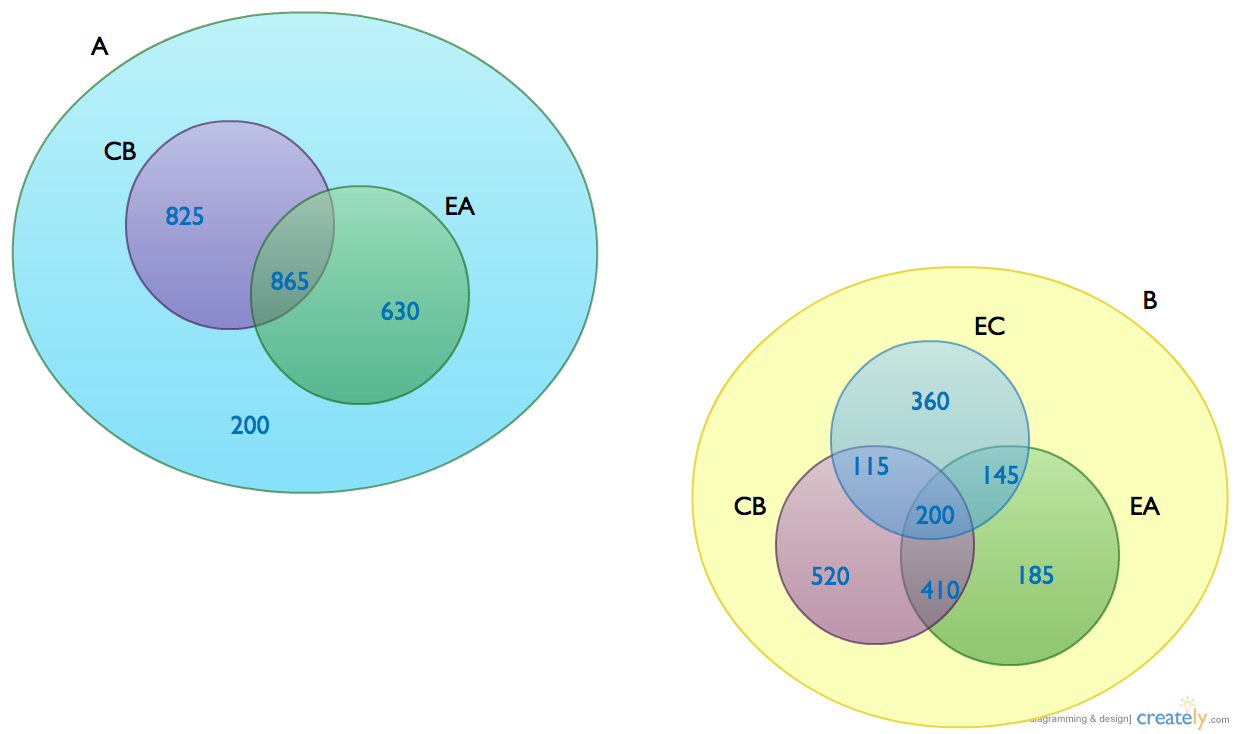
\includegraphics[scale=0.3]{venn_diagram.png}
	\caption{Diagrama de Venn para la representación de probabilidades}
\end{figure}

Las principales cardinalidades para el cálculo de probabilidades son:

$$\left| \Omega \right| = 5000\ \left| A \right| = 2320\ \left| B \right| = 1935\ \left| B^{c} \cap A^{c} \ \right| = 745$$

\item Cuál es la relación entre los eventos, financiarse vía emisión de acciones e invertir en la alternativa B.\\

Los eventos no son mutuamente excluyentes, la probabilidad de su intrsección no es vacía.

$$P(B) = \frac{\left| B \right|}{\left| \Omega \right|} = \frac{1935}{5000} = 0.387$$

$$P(EA) = \frac{\left|  EA \right|}{\left| \Omega \right|} = \frac{\left|  EA \cap A \right| + \left|  EA \cap B \right|}{5000} = \frac{2435}{5000} = 0.487$$

$$P(EA \cap B) = \frac{\left|  EA \cap B \right|}{\left| \Omega \right|} = \frac{185 + 410 + 200 + 145}{5000} = \frac{940}{5000} = 0.188$$

Los eventos son dependientes, pues:

$$P(B)P(EA) = 0.387 \times 0.487 = 0.188 = P(B \cap EA)$$

\item Si se tienen los eventos A y B relacionados con que un accionista esté de acuerdo en invertir en la alternativa A o B, ¿se podría afirmar que estos eventos son independientes? Justifique su respuesta.\\

Los eventos no son independientes, para esto, se listan las probabilidades necesarias:

$$P(A) = \frac{\left| A \right|}{\left| \Omega \right|} = \frac{2320}{5000} = 0.464$$

$$P(B) = \frac{\left| B \right|}{\left| \Omega \right|} = \frac{1935}{5000} = 0.387$$

$$P(B \cap A) = \frac{\left| B \cap A \right|}{\left| \Omega \right|} = \frac{0}{5000} = 0$$

$$P(B \cap A) \neq P(A)P(B)$$

Luego, los eventos no son independientes

\item Calcule la probabilidad de que el accionista esté de acuerdo con invertir en la alternativa B.\\

$$P(B) = \frac{\left| B \right|}{\left| \Omega \right|} = \frac{1935}{5000} = 0.387$$

\item Calcule la probabilidad de que el accionista esté de acuerdo con invertir en la alternativa A y en la alternativa B.\\

$$P(B \cap A) = \frac{\left| B \cap A \right|}{\left| \Omega \right|} = \frac{0}{5000} = 0$$

\item Calcule la probabilidad de que el accionista esté de acuerdo con financiarse vía préstamo bancario.\\

$$P(CB) = \frac{\left| CB \right|}{\left| \Omega \right|} =  \frac{\left| CB \cap A \right|}{\left| \Omega \right|} + \frac{\left| CB \cap B \right|}{\left| \Omega \right|} = 0.587$$

\item Calcule la probabilidad de que el accionista esté de acuerdo con invertir en la alternativa A y que tenga preferencias por obtener un crédito bancario y usar el exceso de caja como posibles métodos de financiación.\\

$$P(A \cap CB \cap EC) = \frac{\left| A \cap CB \cap EC \right|}{\left| \Omega \right|} = \frac{865}{5000} = 0.173$$

\item Calcule la probabilidad de que el accionista esté de acuerdo con financiarse únicamente con una emisión de acciones.\\

Sean los eventos $EA_{A}$ y $EA_{B}$ los eventos que toman sólo la porción que desea invertir únicamente en $EA$ en $A$ y en $B$ respectivamente. $EA_{A} = A \cap (EA \char`\\ (EA \cap CB))$ y $EA_{B} = B \cap (EA \char`\\ (EA \cap CB) \char`\\ (EA \cap EC)$. Se pide la probabilidad de elegir únicamente e tipo $EA$ de financiación, se nombra este evento como $EA_{*}$.

$$P(EA_{*}) = \frac{\left| EA_{*} \right|}{\left| \Omega \right|} = P(EA_{A}) + P(EA_{B}) = \frac{630}{5000} + \frac{185}{5000} =  0.163$$

\item Calcule la probabilidad de que el accionista esté de acuerdo invertir en la alternativa B y tenga preferencias únicamente por dos de los tres métodos de financiación.
$$P(B \cap (CB \cap EC)) + P(B \cap (EA \cap EC)) + P(B \cap (CB \cap EA)) = 0.174$$

\item Si se sabe que el accionista prefiere la inversión en la alternativa B, ¿cuál es la probabilidad de que el accionista tenga preferencias únicamente por las opciones de financiación vía emisión de acciones y préstamo bancario?\\

$$P(EA \cap CB | B) = \frac{\left| EA \cap CB \right|}{\left| B \right|} =  \frac{410}{1935} =  0.211$$

\item Si se sabe que el accionista prefiere financiar el proyecto vía préstamo bancario, ¿cuál es la probabilidad de que el accionista esté de acuerdo en invertir en la alternativa A?\\

$$P(A | CB) = \frac{P(A \cap CB)}{P(CB)} =  \frac{0.338}{0.587} =  0.575$$
\end{enumerate}

\section{Cálculo de probabilidades de eventos (Gráficas)}

Se dispone de un sistema eléctrico que está conformado por 6 componentes, tal como se ilustra en la Figura 2. Este sistema funciona si es posible enviar corriente desde la entrada del sistema hasta su salida. La probabilidad de que cada uno de los componentes funcione apropiadamente es independiente de los demás componentes, y su valor se presenta en la figura que se muestra a continuación, entre paréntesis.

\begin{figure}[h]
\centering
	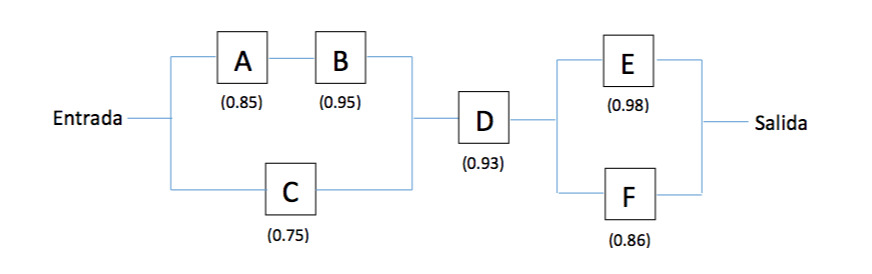
\includegraphics[scale=0.8]{circuit.png}
	\caption{Sistema eléctrico}
\end{figure}

Tenga en cuenta que un sistema en serie funciona si todos sus componentes funcionan; y que un sistema en paralelo funciona si por lo menos uno de los componentes, o serie de componentes, funciona. Con base en la información anterior, responda la pregunta enunciada en el literal $a$.

\begin{enumerate}[(a)]
\item Calcule la probabilidad de que el sistema eléctrico funcione. Sea explícito con el uso de fórmulas, eventos, uniones e intersecciones.\\

Para el desarrollo de este ejercicio, se propone como estrategia reducir cada subsistema mostrado en la Figura 3, y luego hallar la probabilidad de funcionamiento del sistema. Los subsistemas se muestran a continuación.

\begin{figure}[h]
\centering
	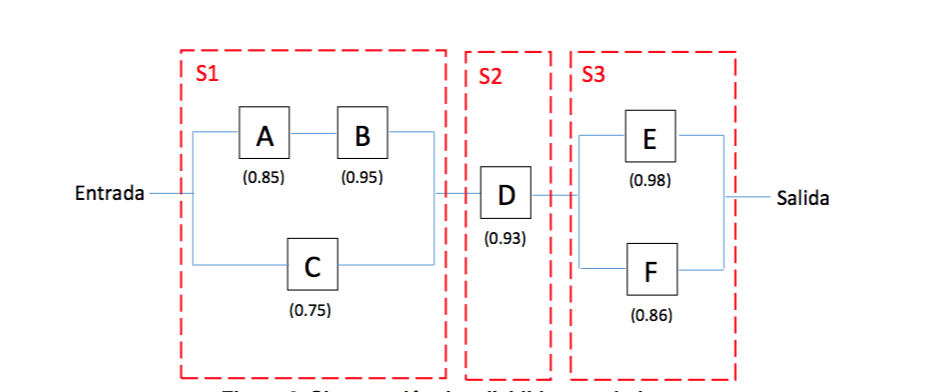
\includegraphics[scale=0.8]{subsystems.png}
	\caption{Sistema eléctrico}
\end{figure}

Para hallar la probabildad de funcionamiento de $S_{1}$, se debe hallar la probabilidad del funcionamiento en serie de $A$ y $B$. A continuación, se halla la probabilidad de funcionamiento de este nuevo bloque con el bloque $C$ en paralelo. El nuevo bloque llamado $A \cap B$, tiene como probabilidad de funcionamiento $P(A \cap B)$. Como cada bloque es independiente, $P(A \cap B) = P(A)P(B)$. Ahora como un sistema en paralelo depende del funcionamiento de al menos uno de los bloques que lo componen, se halla la probabilidad de funcionamiento de los bloques $C$ y $A \cap B$ en paralelo. La probabilidad de funcionamiento de el nuevo bloque llamado $C \cup (A \cap B)$ es $P(C \cup (A \cap B))$, esta probabilidad, se halla con los complementos, es decir, $P(C \cup (A \cap B)) = 1 - P(C^c \cap (A \cap B)^c)$, ya que los eventos son independientes, se tiene $P(C^c \cap (A \cap B)^c) = P(C^c)P((A \cap B)^c)$, esto por la ley de complementos, equivale a $(1 - P(C))(1 - P(A \cap B))$. $P(C \cup (A \cap B)) = P(S_{1})$.

$$P(A \cap B) = P(A)P(B) = (0.85)(0.95) = 0.8075$$
$$P(AB \cup C) = 1 - P(AB^c \cap C^c) = 1 - P(AB^c)P(C^c)$$
$$P(AB \cup C) = 1 - (1 - P(AB))(1 - P(C)) = 1 - (1-0.8075)(1-0.75) = 0.952$$
$$P(S_{1}) =  0.952$$

La probabildad de que el sistema 2 funcione, $P(S_{2})$, es $P(S_{2}) = P(D) = 0.93$. Para el tercer sistema $S_{3}$, se cuenta con dos bloques en paralelo, es decir:

$$P(S_{3}) = P(E \cup F) = 1 - P(E^c \cap F^c) = 1 - P(E^c)P(F^c)$$
$$1 - P(E^c)P(F^c) = 1 - (1 - P(E))(1 - P(F))$$
$$P(S_{3}) =  1 - (1 - 0.98)(1 - 0.86) = 0.997$$

Con las tres probabilidades, $P(S_1), P(S_2), P(S_3)$, se calcula la probabilidad de funcionamiento del sistema. 

$$P(S) = P(S_1 \cap S_2 \cap S_3) = P(S_1)P(S_2)P(S_3) = 0.952 \times 0.93 \times 0.997 =  0.883$$

\end{enumerate}

\section{Técnicas de Conteo}

El próximo torneo de fútbol al que fue invitada la Universidad de los Andes se llevará a cabo en el mes de octubre, y en él competirán 8 equipos. Para este torneo, la Universidad de los Andes contará con la presencia de sus mejores cuatro equipos, pertenecientes a las facultades de Ingeniería, Administración, Derecho y Matemáticas. Los restantes cuatro equipos, provenientes de otras universidades, pertenecen a las facultades de Ingeniería, Comunicación, Psicología y Diseño.\\

Los organizadores del torneo aún no han informado cuál es el sistema de eliminación, sin embargo, usted supone que se implementará un sistema de puntos en el que todos juegan contra todos. Conteste las siguientes preguntas bajo el supuesto de que es un torneo en el que todos juegan
contra todos.

\begin{enumerate}[(a)]
\item ¿Cuántos resultados posibles se pueden dar en términos de los puestos obtenidos
por cada equipo?

$$8 \times 7 \times 6 \times 5 \times 4 \times 3 \times 2 \times 1 = 40320$$

\item ¿Cuál es la probabilidad de que el primer y el segundo puesto sean ocupados por
equipos de los Andes?

$$P(A) = \frac{|A|}{|\Omega|} = \frac{2! \times 6P6}{40320} = \frac{2! \times 8640}{40320}$$

\item ¿Cuál es la probabilidad de que los tres primeros lugares sean ocupados por equipos
de las facultades de Comunicación, Derecho y Administración (sin importar el orden)?

$$P(A) = \frac{|A|}{|\Omega|} = \frac{3P3 \times 5P5}{40320} = \frac{120}{40320} = 0.0178$$

\item ¿Cuál es la probabilidad de que el primer lugar sea ocupado por un equipo de
Ingeniería, el segundo por el de Matemáticas y el tercero por el de Diseño?

$$P(A) = \frac{|A|}{|\Omega|} = \frac{2P1 \times 1 \times 5P5}{40320} = \frac{240}{40320} = 0.00595238$$
\end{enumerate}



Su otro supuesto sobre el sistema de eliminación consiste en que se organizarán dos grupos de
cuatro equipos, y se realizará una ronda final entre los ganadores de cada uno de los grupos. Bajo
este supuesto, de respuesta a las siguientes preguntas.

\begin{itemize}
\item[(e)] ¿De cuántas formas distintas se podrían organizar los 8 equipos en dos grupos?

$$\binom{8}{4} \times \binom{4}{4} = 70$$

\item[(f)]  ¿Cuál es la probabilidad de que en un mismo grupo quede únicamente un equipo de
Ingeniería y el equipo de Diseño?

$$\frac{\binom{2}{1}\binom{1}{1}\binom{5}{2}\binom{3}{3}}{\binom{8}{4}}$$

\item[(g)]  Si se supone que los cuatro equipos representantes de la Universidad de los Andes
quedan en el mismo grupo ¿Cuál es la probabilidad de que los equipos de las facultades de
Ingeniería queden de primeros en cada grupo?

$$\frac{3!}{4!} \times \frac{1}{4}$$
\end{itemize}

\section{Teorema de Bayes y Árboles de Probabilidad}

Luego del impresionante duelo que se vio entre el ciclista británico Chris Froome y el colombiano
Nairo Quintana en el Tour de Francia 2015, ambos podrían volver a enfrentarse el próximo 22 de
agosto en la 70ª edición de la Vuelta Ciclística a España. Conocedores del trazado han analizado
que, de las 21 etapas que conforman los 3,374.4 kilómetros de la Vuelta, hay 3 en especial que se podrían considerar decisivas para coronarse en Madrid. Según datos históricos, el ganador de la Vuelta únicamente ha necesitado acumular dos victorias en cualquiera de las siguientes tres etapas para sacar suficiente ventaja sobre el segundo:

\begin{itemize}
\item Etapa 11: Andorra – Els Cortals d’Encamp. 138 km. Considerada como la etapa más dura de la historia del evento, cuenta con seis puertos de montaña en 138 km que suman 5,230 metros de desnivel acumulado.
\item Etapa 16: Luarca – Ermita del Alba. 184 km. Esta etapa consta de siete puertos, quizá no de la dificultad de los dispuestos en la 11ª, pero con dos semanas encima de carrera el cansancio empieza a influir. A su vez, la trazada presenta curvas en herradura, muros de más del 20\% durante más de 2000 metros.
\item Etapa 20: San Lorenzo de El Escorial – Cercedilla. 181 km. Esta será la etapa de cierre de la vuelta con puertos ya bastante conocidos como Navacerrada, Cotos o La Morcuera pero sin final en alto. Este será el terreno definitivo para que, después de tres semanas de actividad, se definan los primeros puestos de la vuelta.
\end{itemize}

Según estimaciones realizadas por expertos, la probabilidad de que Nairo gané en la 11ª Etapa de
la Vuelta es de 0.65; y, suponiendo que Nairo ganó dicha etapa, la probabilidad de que también gane
la 16ª es de 0.7. Por otro lado, si Froome gana la 11ª Etapa, la probabilidad de que gane la 16ª sería
de 0.5.\\

Los analistas estiman que si alguno de los dos gana las etapas 11 y 16, se proclamará como el
ganador de la vuelta a España, sin importar el resultado de la 20ª Etapa. Pero, en caso de que no
se defina el título en las etapas 11 y 16, el ganador se definirá en la 20ª Etapa, antes de llegar a
Madrid, para la cual los dos ciclistas tienen igual probabilidad de ganarla. Asumiendo que cada etapa es independiente de las otras y que únicamente Nairo y Froome las podrían ganar, responda las siguientes preguntas.

\begin{enumerate}[(a)]

\item Construya un árbol de probabilidad que represente la situación descrita.\\ 

Los eventos dispuestos son:

$N_i$ es el evento de que Nairo gane el $i$-ésimo evento. Por lo tanto, $N_{i}^c$ es que Froome gane la misma etapa.  $N$ es que Nairo gane la vuelta a España. Las probabilidades deducidas a partir del enunciado son:

$$P(N_1) = 0.65 \ P(N_2 | N_1) = 0.65 \ P(N_2 | N_{1}^c) = 0.65$$

El arbol de probabilidad se muestra en la Figura 4.

\begin{figure}[h]
\centering
	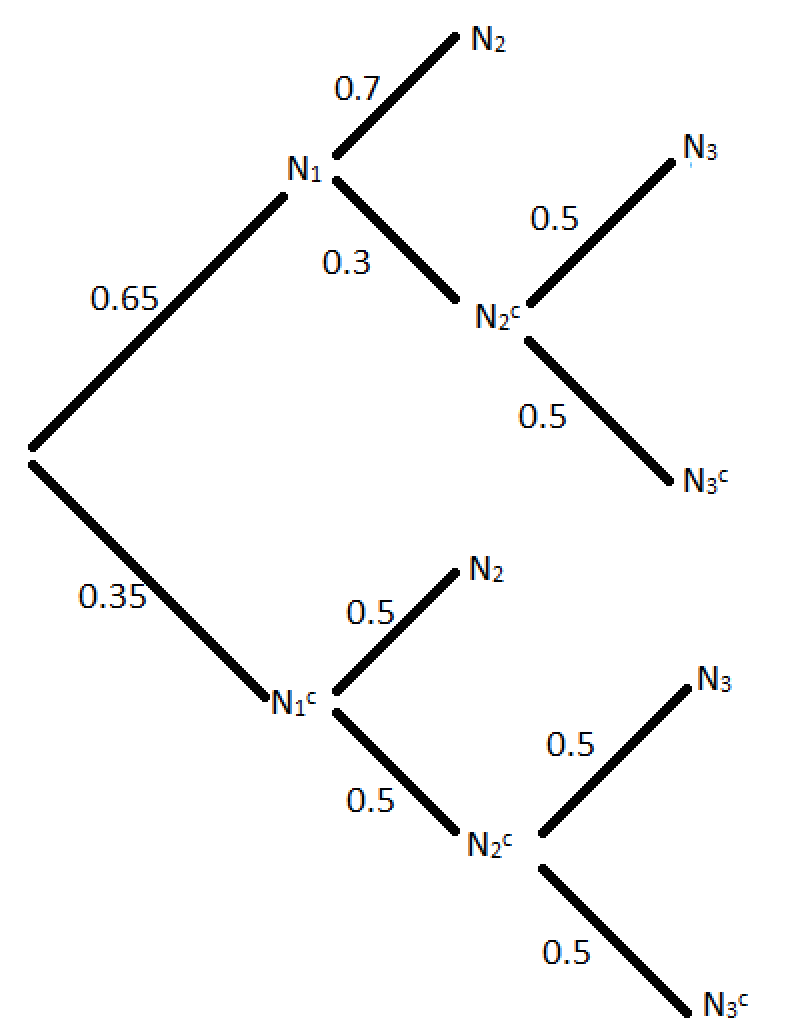
\includegraphics[scale=0.5]{tree.png}
	\caption{Diagrama de Venn para la representación de probabilidades}
\end{figure}

\item ¿Cuál es la probabilidad de que Nairo Quintana gane la Vuelta a España? ¿Cuál es
la probabilidad de que Chris Froome gane la Vuelta a España?

$$P(N) = P(N_2) + P(N_3 \cap N_2^c \cap N_1) + P(N_3 \cap N_2 \cap N_1^c)$$
$$P(N) = 0.455 + 0.0975 + 0.0875 = 0.64$$

$$P(N^c) = P(N_2^c) + P(N_3^c \cap N_2^c \cap N_1) + P(N_3^c \cap N_2 \cap N_1^c)$$
$$P(N^c) = 0.175 + 0.0975 + 0.0875 = 0.36$$


\item ¿Cuál es la probabilidad de que el ganador de la Vuelta se haya coronado ganando
las etapas 11ª y 16ª?

$$P(C) = P(N_2 \cap N_1) + P(N_2^c \cap N_1^c) = 0.455 + 0.175 = 0.63$$

\item Si se sabe que Froome ganó la 16ª etapa, ¿cuál es la probabilidad de que haya
ganado la 11ª?

$$P(N_1^c | N_2^c) = \frac{P(N_1^c \cap N_2^c)}{P(N_2^c)} = \frac{P(N_2 | N_1)P(N_1)}{P(N_2^c)}$$

$$P(N_2^c) = P(N_2^c | N_1)P(N_1) + P(N_2^c | N_1^c)P(N_1^c) = (0.3)(0.65) + (0.5)(0.35)$$
$$P(N_2^c) = 0.37$$
$$P(N_1^c | N_2^c) = 0.473$$

\end{enumerate}

\section{Variables Aleatorias Discretas}

Alberto y sus amigos han diseñado un juego de azar que consiste en lanzar 2 dados al tiempo y
luego sacar una bola de una urna que contiene 3 bolas blancas, 3 rojas y 3 negras. La apuesta de este juego son 10 dólares, y cada participante debe elegir un número del 1 al 6 y un color entre blanco, rojo y negro. Las reglas del juego son las siguientes:

\begin{itemize}
\item Si no se obtiene el número elegido en ninguno de los dados, sin importar si se adivinó el
color de la bola, el jugador pierde lo apostado.

\item Si el número elegido sale en 1 de los 2 dados y no se saca la bola del color seleccionado,
se recibe lo apostado y no se pierde dinero.

\item Si el número elegido sale en 1 de los 2 dados y se saca la bola del color seleccionado, se
recibe el doble de lo apostado.

\item Si el número sale en los 2 dados y no se saca la bola del color seleccionado se recibe 5
veces lo apostado.

\item Si el número sale en los 2 dados y se saca la bola del color seleccionado se recibe 8 veces
lo apostado.
\end{itemize}

Se define $X$ como la variable aleatoria que representa la ganancia o pérdida neta del juego.
Responda los siguientes literales:

\begin{enumerate}[(a)]

\item Encuentre la Función de Probabilidad de la variable aleatoria $X$ y grafíquela.\\

Sea $X$ la variable aleatoria para modelar el experimento, el rango de la ganancia o pérdida o el dinero obtenido es $R[X] = [-10, 0, 10, 40, 70]$. La probabilidad de obtener cada punto dentro del rango, se obtiene usando contéo.

$$P(X = -10) = \frac{5 \times 5 \times 9}{6 \times 6 \times 9} = 0.69$$
$$P(X = 0) = \frac{1 \times 5 \times 6}{6 \times 6 \times 9} = 0.185$$
$$P(X = 10) = \frac{2 \times 1 \times 5 \times 3}{6 \times 6 \times 9} = 0.0925$$
$$P(X = 40) = \frac{1 \times 1 \times 5}{6 \times 6 \times 9} = 0.0185$$
$$P(X = 70) = \frac{1 \times 1 \times 3}{6 \times 6 \times 9} = 0.0092$$

La función de probabilidad de la variable aleatoria $X$ es:

\begin{equation}
f_X(x) =  
\[ \begin{cases} 
	  0.69 & x = -10 \\ 
	  0.185 & x = 0 \\ 
	  0.0925 & x = 10 \\ 
	  0.0185 & x = 40 \\ 
	  0.0092 & x = 70
   \end{cases}
\]
\end{equation}

\begin{figure}[h]
\centering
	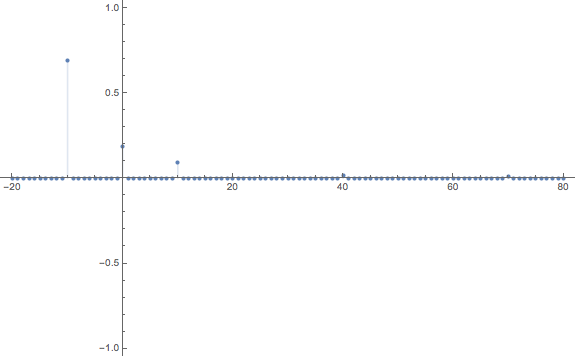
\includegraphics[scale=0.6]{pdf_discrete.png}
	\caption{Distribución de probabilidad}
\end{figure}

\pagebreak

\end{enumerate}

\begin{enumerate}[(b)]
\item Encuentre la Función de Distribución Acumulada de la variable aleatoria $X$ y
grafíquela.

La función de distrnución acumulada de la variable aleatoria $X$ es:

\begin{equation}
F_X(x) =  
\[ \begin{cases} 
	  0.69 & x \leq -10 \\ 
	  0.875 & -10 < x \leq 0 \\ 
	  0.9675 & 0 < x \leq 10 \\ 
	  0.986 & 10 < x \leq 40 \\ 
	  0.99 & 40 < x \leq 70 	\\	
	  1 & x > 70
   \end{cases}
\]
\end{equation}

\begin{figure}[h]
\centering
	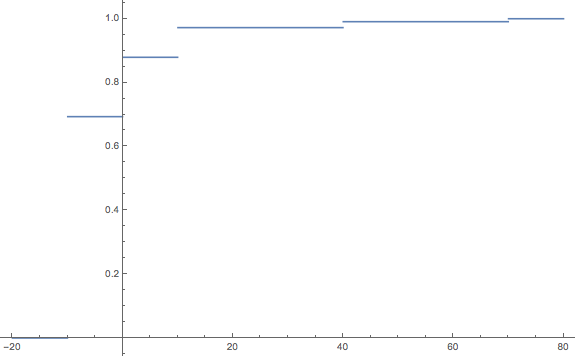
\includegraphics[scale=0.6]{pcf_discrete.png}
	\caption{Distribución de probabilidad}
\end{figure}

\pagebreak

\end{enumerate}

\begin{enumerate}[(c)]
\item Calcule el valor esperado y la desviación estándar de la variable aleatoria $X$.
Interprete sus resultados.\\

$$E[X] = \sum_{x_{i} \in R[X]} x_{i} \times f_{X}(x_{i})$$
$$E[X] = (-10)(0.69) + (0)(0.0185) + (10)(0.0925) + (40)(0.0185) + (70)(0.0092)$$
$$E[x] = -4.58$$

$$Var[X] = E[X^2] - (E[X])^2 = 132.2$$
$$Des[X] = \sqrt{132.2}$$

En promedio, se espera perder tras participar en el experimento aleatorio.

\end{enumerate}

\begin{enumerate}[(d)]
\item ¿Cuál es la probabilidad de generar ganancia en el juego? Interprete el resultado.

$$P(X > 0) =  1 - P(X \leq 0) = 1 - (P(X = 0) + P(X = -10))$$
$$P(X > 0) =  1 - P(X \leq 0) = 1 - (0.185 + 0.69) = 0.125$$
\end{enumerate}

\section{Variables Aleatorias Continuas}

La nueva junta administrativa del Hospital Santa Concepción está interesada en desarrollar nuevas estrategias para implementar el próximo año, que permitan mejorar el nivel de servicio que se ofrece a sus pacientes. En la pasada reunión se decidió que el hospital requiere prestar más atención a los tiempos de espera de los pacientes ambulatorios. Como base para la toma de decisiones encaminadas a mejorar en este aspecto, la junta realizó un acuerdo con la Universidad de los Andes para que se realice una evaluación de las salas de espera en el hospital. Luego de casi seis meses de toma de tiempos y análisis estadístico, los investigadores de la universidad lograron caracterizar el tiempo, en horas, que un paciente ambulatorio debe esperar antes de ser atendido como una variable aleatoria X cuya función de densidad de probabilidad está dada por:

\begin{equation}
f_X(x) = 
\[ \begin{cases} 
      x^2 & 0 \leq x < 1 \\      
      k & 1 \leq x < \frac{4}{3} \\      
      -\frac{3x}{2} + 3 & \frac{4}{3} \leq x < 2 \\
      0 & d.l.c. 
   \end{cases}
\]
\end{equation}

\begin{enumerate}[(a)]

\item ¿Cuál es el valor de la constante k que garantiza que la función de densidad de
probabilidad de la variable aleatoria X esté correctamente definida? Realice la gráfica de la
distribución de probabilidad.\\

Para esto, la sumatoria de la función $f_X(x)$, debe ser igual a 1.

\begin{equation}
\int f_X(x) dx = 1
\end{equation}

\begin{equation}
\left( \int_{0}^{1} x^2 \ dx \right) + \left( \int_{1}^{\frac{4}{3}} k \ dx \right) + \left( \int_{\frac{4}{3}}^{2} -\frac{3x}{2} + 3 \ dx \right) = 1
\end{equation}

\begin{equation}
\frac{1}{3} + \frac{k}{3} + \frac{1}{3} = \frac{2}{3} + \frac{k}{3} = 1 \Rightarrow k = 1
\end{equation}

La función de probabilidad queda de la siguiente manera:

\begin{equation}
f_X(x) = 
\[ \begin{cases} 
      x^2 & 0 \leq x < 1 \\      
      1 & 1 \leq x < \frac{4}{3} \\      
      -\frac{3x}{2} + 3 & \frac{4}{3} \leq x < 2 \\
      0 & d.l.c. 
   \end{cases}
\]
\end{equation}

La gráfica es:

\begin{figure}[h]
\centering
	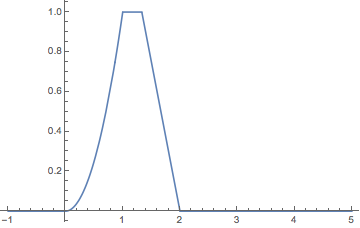
\includegraphics[scale=0.6]{pdf_continuous.png}
	\caption{Distribución de probabilidad}
\end{figure}

\begin{enumerate}[(b)]
\item Halle la función de distribución acumulada del tiempo de espera de un paciente
ambulatorio en el hospital y grafíquela.\\

La función de distribución acumulada, queda así:\\

\begin{equation}
F_X(x) = \int_{- \infty}^{x} f_X(x) dx =  
\[ \begin{cases} 
	  0 & x < 0 \\
      \frac{x^3}{3} & 0 \leq x < 1 \\      
      x - 1 & 1 \leq x < \frac{4}{3} \\      
      - \frac{3x^2}{4} + 3x - \frac{8}{3} & \frac{4}{3} \leq x < 2 \\
      1 & x \geq 2 
   \end{cases}
\]
\end{equation}

La gráfica es:.

\begin{figure}[h]
\centering
	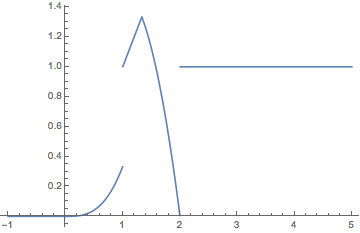
\includegraphics[scale=0.5]{pcf_continuous.png}
	\caption{Distribución de probabilidad}
\end{figure}


\end{enumerate}
\begin{enumerate}[(c)]
\item ¿Cuánto tiempo se espera que un paciente ambulatorio del hospital debería esperar
antes de ser atendido? ¿Cuánto sería la desviación estándar de dicho tiempo de espera?\\

Se pregunta por el valor esperado y la desviación estándar de la distribución.

$$E[X] = \left( \int_{0}^{1} x \times x^2 \ dx \right) + \left( \int_{1}^{\frac{4}{3}} x \times 1 \ dx \right) + \left( \int_{\frac{4}{3}}^{2} x \times (-\frac{3x}{2} + 3) \ dx \right)$$
$$E[X] = 1.15741 H$$

$$E[X^2] = \left( \int_{0}^{1} x^2 \times x^2 \ dx \right) + \left( \int_{1}^{\frac{4}{3}} x^2 \times 1 \ dx \right) + \left( \int_{\frac{4}{3}}^{2} x^2 \times (-\frac{3x}{2} + 3) \ dx \right)$$
$$E[X^2] = 1.4716$$

$$Var[X] = E[X^2] - (E[X])^2 = 1.4716 - (1.15741)^2 = 0.132002$$
$$Desv[X] = \sqrt{Var[X]} = \sqrt{0.132002} = 0.363321$$

\end{enumerate}
\begin{enumerate}[(d)]
\item Si se selecciona un paciente del hospital al azar, ¿cuál es la probabilidad de que este
deba esperar exactamente una hora para ser atendido?\\

Dado que es una distribución continua, la integral es cero para los dos intervalos de integración iguales, es decir, en puntos específicos del rango, la probabilidad tiende a cero. $P(X = 1) = 0$

\end{enumerate}
\begin{enumerate}[(e)]
\item Calcule la probabilidad de que un paciente seleccionado al azar deba esperar entre
1.25 y 1.75 horas antes de ser atendido. Grafique la región correspondiente.\\

$$P(1.25 < X < 1.75) = \int_{1.25}^{1.75} -\frac{3x}{2} + 3 \ dx = 0.375$$
\end{enumerate}

\begin{enumerate}[(f)]
\item Si se sabe que el tiempo de espera será superior a 1 hora, Calcule la probabilidad
de que un paciente seleccionado al azar deba esperar entre 1.25 y 1.75 horas antes de ser
atendido.\\

$$P(1.25 < X < 1.75 \ | \ X > 1) = \frac{P((1.25 < X < 1.75) \cap (X > 1))}{P(X > 1)}$$

Ya que los trozos de tiempo $1.25 < X < 1.75$ y $X > 1$ se traslapan, su intersección es el pedazo en común, ya que el pedazo $1.25 < X < 1.75$, $X$ toma un valor mayor a uno, esta es la intersección.

$$P(1.25 < X < 1.75 \ | \ X > 1) = \frac{P(1.25 < X < 1.75)}{P(X > 1)} = \frac{P(1.25 < X < 1.75)}{1 - P(X < 1)}$$

$$P(1.25 < X < 1.75 \ | \ X > 1) = \frac{0.375}{1 - P(X < 1)} = \frac{0.375}{1 - \int_{- \infty}^{1} f_X(x)}$$

$$P(1.25 < X < 1.75 \ | \ X > 1) = \frac{0.375}{1 - \int_{0}^{1} x^2}$$

\end{enumerate}




\end{document}